\documentclass[12pt]{article}

\usepackage{subcaption} 
\usepackage{amsmath,graphicx,amssymb}
\usepackage{units}
\usepackage{setspace}
\usepackage{esint}
\usepackage{pgfplots}
\usepackage{listings}
\usepackage{accents}
\usepackage{hyperref}
\usepackage{float}
\pgfplotsset{width=8cm,compat=1.9}

\usepackage{color} %red, green, blue, yellow, cyan, magenta, black, white
\definecolor{mygreen}{RGB}{28,172,0} % color values Red, Green, Blue
\definecolor{mylilas}{RGB}{170,55,241}

\usepackage[letterpaper, portrait, margin=.75in]{geometry}
\usepackage{amsmath}

\title{Julia Sets}
\author{Tyler Klein\and Ben Zager\and Jack O'Shea}
\allowdisplaybreaks
\renewcommand{\baselinestretch}{1.5}

\newcommand{\pard}[2]{\frac{\partial #1}{\partial #2}}
\newcommand{\cross}[2]{\vec{#1}\times\vec{#2}}
\newcommand{\vspacee}[1]{\newline\vspace{#1}\newline}
\newcommand{\DS}{\Delta S}
\newcommand{\atml}{\hspace{1mm}atm \cdot L}
\newcommand{\R}{.0821\frac{atm\cdot L}{mol\cdot K}}
\newcommand{\dbar}[1]{\bar{\underaccent{\bar}{#1}}}
\newcommand{\pmf}[1]{P_{\dbar{\MakeUppercase{#1}}}(\MakeLowercase{#1})}
\newcommand{\labelPoint}[2]{\node [above] at (axis cs: #1,#2 ) {(#1,#2)};
	\draw[red,fill=red](axis cs:  #1,  #2) circle[radius=2pt];}

\begin{document}
\lstset{language=Matlab,%
	%basicstyle=\color{red},
	breaklines=true,%
	morekeywords={matlab2tikz},
	keywordstyle=\color{blue},%
	morekeywords=[2]{1}, keywordstyle=[2]{\color{black}},
	identifierstyle=\color{black},%
	stringstyle=\color{mylilas},
	commentstyle=\color{mygreen},%
	showstringspaces=false,%without this there will be a symbol in the places where there is a space
	numbers=left,%
	numberstyle={\tiny \color{black}},% size of the numbers
	numbersep=9pt, % this defines how far the numbers are from the text
	emph=[1]{for,end,break},emphstyle=[1]\color{red}, %some words to emphasise
	%emph=[2]{word1,word2}, emphstyle=[2]{style},    
}
	
	
\maketitle
\section*{Introduction}
Julia sets are sets of complex numbers that do not converge to a point when iterated upon by a given map. When computed and plotted using various algorithms, these sets often produce very beautiful images, sometimes fractals, in the complex plane. The case most often studied is functions of the form $f(Z)= Z^2+C$, where Cis any number in the complex plane. In our project, we studied two function groups: functions of the form $f(Z)= Z^n+C$, and variations of Newton’s method.
%%%%%%%%%%%%%%%%%%%%%%%%%%%%%%%%%%%%%%%%%%%%%
\section*{Intuitive  Explanation for Fractal Formation}
Computer researcher Karl Sims offers an extremely intuitive explanation of why fractals in the complex plane result from these iterative functions. The following explanation and images are adapted from his work at: http://www.karlsims.com/julia.html
Instead of using the equation $z=z^2+c$ , we'll transform it by subtracting c from both sides and taking the square root. Now our equation looks like $z=\pm\sqrt{z-c}$  and we can apply this to a set of points in the complex plane to generate the shape of the Julia set. We will use the disk of radius 2 centered at the origin of the complex plane as our set. Note the red dot represents the origin and it is assumed the reals lay along the horizontal axis and the imaginaries on the vertical.
\begin{figure}[H]
	\centering
	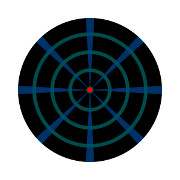
\includegraphics[width=0.2\linewidth]{images/julia0}
	\label{fig:rootEx2}
\end{figure}
We begin to carry out the transformation $z=\pm\sqrt{z-c}$ by first applying the translation transformation inside the square root function, subtracting the complex number c from each point in the set. Using a c value of $.274 - .008$i means we will shift each point on the disk .274 units left (along the real axis), and only slightly up (0.008 units along the imaginary axis)
\begin{figure}[H]
	\centering
	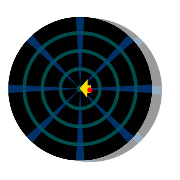
\includegraphics[width=0.2\linewidth]{images/julia1}
	\label{fig:rootEx2}
\end{figure}
The next step is applying the square root function to the set. The first effect of this transformation is halving the angle between all points and the positive real axis
\begin{figure}[H]
	\centering
	\begin{subfigure}{.5\textwidth}
		\centering
		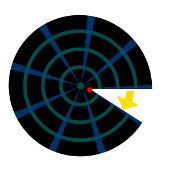
\includegraphics[width=.4\linewidth]{images/julia2}
		\label{fig:sub1}
	\end{subfigure}%
	\begin{subfigure}{.5\textwidth}
		\centering
		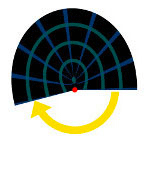
\includegraphics[width=.4\linewidth]{images/julia3}
		\label{fig:sub2}
	\end{subfigure}
	\label{fig:test}
\end{figure}
The square root function produces positive and negative results, but the figures above only shows the positive result. The following transformation also occurs and produces the negative half of the set
\begin{figure}[H]
	\centering
	\begin{subfigure}{.5\textwidth}
		\centering
		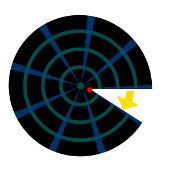
\includegraphics[width=.4\linewidth,angle=180]{images/julia2}
		\label{fig:sub1}
	\end{subfigure}%
	\begin{subfigure}{.5\textwidth}
		\centering
		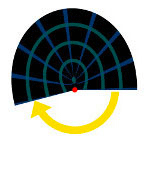
\includegraphics[width=.4\linewidth,angle=180]{images/julia3}
		\label{fig:sub2}
	\end{subfigure}
	\label{fig:test}
\end{figure}
These two resulting sets are merged to form
\begin{figure}[H]
	\centering
	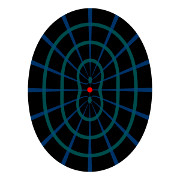
\includegraphics[width=0.2\linewidth]{images/julia4}
	\label{fig:rootEx2}
\end{figure}
The square root function also halves the distance between any point in the complex 
plane and the origin, so the final step in this iteration is to shrink the above set by a factor of 2.
\begin{figure}[H]
	\centering
	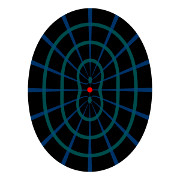
\includegraphics[width=0.1\linewidth]{images/julia4}
	\label{fig:rootEx2}
\end{figure}
The first iteration is now complete, and we restart the process beginning with the figure above instead of the disk with radius 2
\begin{figure}[H]
	\centering
	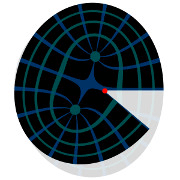
\includegraphics[width=.2\textwidth]{images/julia6}\hfill
	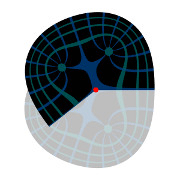
\includegraphics[width=.2\textwidth]{images/julia7}\hfill
	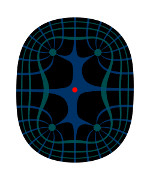
\includegraphics[width=.2\textwidth]{images/julia8}
	\label{fig:figure3}
\end{figure}
The following figures are the results of 3, 6, 30, and 100 iterations, respectively
\begin{figure}[H]
	\centering
	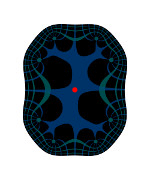
\includegraphics[width=.2\textwidth]{images/julia9}\hfill
	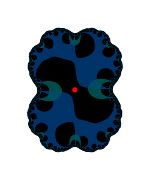
\includegraphics[width=.2\textwidth]{images/julia10}\hfill
	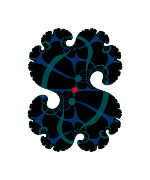
\includegraphics[width=.2\textwidth]{images/julia11}\hfill
	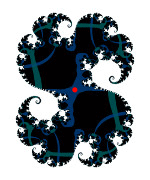
\includegraphics[width=.2\textwidth]{images/julia12}
	\label{fig:figure3}
\end{figure}
You may notice that the function used to produce these graphical representations of the Julia Set for $f(z)$ is actually the inverse of $f$. This process certainly differs from the typical algorithm used to generate the figures, but the end result is the same. 
Let $\mathbf{J}$ denote the Julia Set of our function, $C$ denote the complex plane, and $D$ denote the disk of radius 2 in the complex plane. Typically we generate $\mathbf{J}$ by applying the map $f:~C\rightarrow~C$ such that $f(z)=\lim\limits_{z\rightarrow\infty}z_k$ where $z_k=z^2_{k-1}+c$  to some subset of $C$ that we guess contains $\mathbf{J}$, (let’s call this $C’$). We begin mapping each $z\in C'$ and if $f(z)\in D$  we say $z\in\mathbf{J}$ . The domain and codomain of this algorithm is denoted $~C$ because as we test more points of $C’$, we can use our results to eliminate other points of $C’$ without explicit testing them. As our algorithm progresses, the domain tends towards $\mathbf{J}$. With the inverse function, however, we can properly state the domain and codomain from the start: $f^{-1}:D\rightarrow J$ such that $f^{-1}(z)=\lim\limits_{k\rightarrow\infty}z_k$ where $z_k=\sqrt{z_{k-1}-c}$ . The image of $f^{-1}(D)$ is clearly $\mathbf{J}$ because for any $z\in D$, $f(f^{-1}(z))=z$ and $z\in D=$ the disk of radius 2 centered at the origin, which is exactly how we define an element of a Julia Set.
What is this explanation useful for? It can help us predict the shape of some Julia Sets before creating them, and have a better understanding of why certain c value result in fractals with certain symmetries. 
When $c=0$, all points diverge except for the origin. The process above offers another method for understanding why this is true. Take the disk of radius 2 and simply rotate it in place, then shrink it around the origin. Repeating this process infinite times yields the Julia Set, a disk with an infinitely small radius, that only contains the origin.
When the imaginary component of $c$ is 0, there will be no vertical translation of D before the “rotation”, so the Julia set will be symmetric about the horizontal or real axis.
%%%%%%%%%%%%%%%%%%%%%%%%%%%%%%%%%%%%%%%%%%
\section*{Simple Polynomials}
For polynomials of the form $f(Z)= Z^n+C$, the function was applied repeatedly to a grid of points in the complex plane centered at the origin. Before each iteration, each point was checked to see if it was outside of the escape radius. The escape radius is a radius beyond which points cannot possibly converge to a root. This is due to the fact that beyond the radius, each iteration takes the point further away from the origin, without bound. As a result, we know that all points outside of this radius won’t converge. The iteration at which points cross the radius is stored and used for plotting. The escape radius for these functions can be derived quite easily, as shown below.
%%%%%%%%%%%%%%%%%%%%%%%%%%%%%%%%%%%%%%%%%%%%%%%%%%%%%%%%%
\begin{onehalfspace}
	Let $f(z)=z^n+C$
	\begin{flalign*}
	&&|f(z)|&=|z^n+C|&&\\
	&&\frac{|f(z)|}{|z|}&=\frac{|z^n+C|}{|z|}&&\\
	\hspace{45mm}&&|z^n+C|&\geq|z^n|-|C|&&\footnotesize\text{via triangle theorem}\normalsize\\
	&&\frac{|f(z)|}{|z|}&\geq\frac{|z^n|-|C|}{|z|}&&\\
	&&\frac{|f(z)|}{|z|}&\geq\frac{|z|^n-|C|}{|z|}&&\footnotesize\text{via Proof 1}\normalsize\\
	&&\frac{|f(z)|}{|z|}&\geq|z|^{n-1}-\frac{|C|}{|z|}&&\\
	&&|z|^{n-1}-\frac{|C|}{|z|}&\geq |z|^{n-1}-1 \hspace{2mm}\text{    when }\hspace{3mm}|z|\geq|C|&&\\
	&&|z|^{n-1}-1&\geq 1 \hspace{2mm}\text{    when }\hspace{3mm}|z|^{n-1}\geq|2|&&\\
	&&\huge\therefore\normalsize\frac{|f(z)|}{|z|}\geq1\hspace{4mm}\text{when}&\hspace{4mm}|z|\geq\sqrt[n-1]{2}\geq|C|&&\\
	\end{flalign*}
	As a result, the point grows rapidly when $|z|\geq\sqrt[n-1]{2}$, so we know all points that lead to an iteration that has a magnitude above $\sqrt[n-1]{2}$, the sequence diverges.\\ \vspace{1mm}
\subsubsection*{Iteration Grid Code}
	Our code works by first creating an equally spaced grid of points using the \verb|meshgrid| command in Matlab. We declare a center point, the origin, the distance and the step size, and use meshgrid to create two matrices that can be added together to create a grid.
	\begin{lstlisting}
		x=linspace(xcen-d,xcen+d,points);
		y=linspace(ycen-d,ycen+d,points);
		[x,y]=meshgrid(x,y); %creates 2 matrices
		z = x+1i.*y;
	\end{lstlisting}
	The escape radius is then calculated, and the for loop is executed.
	\begin{lstlisting}
		escapeRadius = nthroot(2,powerN-1);
		for iter=0:iters
			escaped = abs(z)>escapeRadius; % particles that "escaped"
			z(escaped) = NaN; % prevent further iterations
			kGrid(escaped) = iter;    
			z=func(z); % apply mapping
		end
	\end{lstlisting}
	Inside the for loop, the function first checks if any points have escaped, and if so, it denotes the iteration after which the point escaped. Then, the points are set to NaN, so the program ignores them for future calculations. All of the points outside the escape radius automatically have a value of 0, since they are escaped before any iteration takes place. The function then applies the mapping for the next iteration, then repeats. The program then returns \verb|kGrid|, which is the grid of the iterations after which each point escape (if it didn't escape, it's value is 0). These values will be refered to as the 'K-values' from now on.
%%%%%%%%%%%%%%%%%%%%%%%%%%%%%%%%%%%%%%%%%%%%%%%%%%%%
\subsubsection*{Plotting Code}	
To plot the K-values, we created a function that takes the grid of K-values, and generates an image using \verb|imagesc|. This command generates an image from a matrix of values using scaled colors. Since our grid has only 1 number, we use a colormap to ensure we have interesting color schemes. The script includes some auto-naming of plots, saving capabilities, and other small features. Here are some images generated using the two functions in combination.
\begin{figure}[H]
	\centering
	%\includegraphics[width=.7\linewidth]{"images/im1"}
	\caption{Fractal for C=$.8i$}
	\label{fig:}
\end{figure}
\begin{figure}[H]
\centering
\includegraphics[width=.7\linewidth]{"images/sweep1"}
\caption{Sweep of C values}
\label{fig:untitled3}
\end{figure}
%%%%%%%%%%%%%%%%%%%%%%%%%%%%%%%%%%%%%%%%%%%
\section*{Newton’s Method for Generating Julia Sets}
Newton’s method is a root finding technique that is a special case of fixed point iteration, in the form of  $x_{k+1}=x_k - \frac{f(x)}{f'(x)}$,  with an initial approximation, $x0$.  Newton’s method can converge quadratically with an initial guess that is “close enough”, as long as the derivative at the root is not zero.  By applying Newton’s method to functions of the form $f(z) = z^n + c$,  on a set of points in the complex plane, we can generate a special case of Julia sets called Newton fractals.  As we will see, the complicated dynamics of Newton fractals provides some insight on the convergence of Newton’s method, and how it can be affected by initial guesses and roots of higher multiplicity.  There  are two main methods for creating Newton fractals.  The first method maps a starting point to the root where it converges.  The other method maps a starting point to the number of iterations required for convergence, up to some given tolerance.   We will start by discussing the first method.
\subsubsection*{Mapping by root}
\begin{figure}[H]
\centering
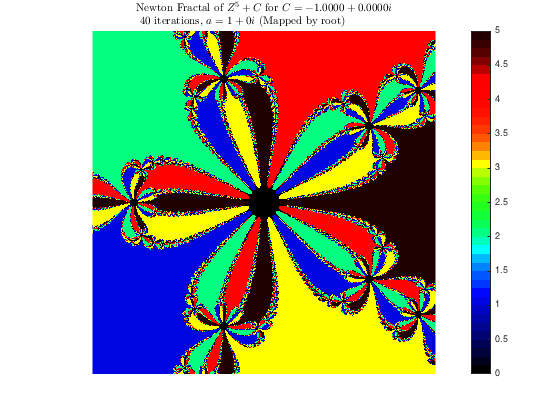
\includegraphics[width=0.7\linewidth]{images/rootEx2}
\caption{}
\label{fig:rootEx2}
\end{figure}
The basins of attraction for Newton’s method are defined as the regions  for which all initial guesses will converge to a single root.  According to a result discovered by Arthur Cayley, if a complex quadratic polynomial has roots $\alpha$ and $\beta$, and $L$ is the perpendicular bisector of the line segment joining those roots, then the basins of attraction for which Newton’s method will converge to either $\alpha$ or $\beta$ are the half planes into which $L$ divides the complex plane.  This means that an initial approximation $z_{0}$ will only converge to $\alpha$ if $|z_{0} - \alpha| < |z_{0} - \beta|$.  If $z_{0}$ lies on $L$, then Newton’s method will not converge.  For polynomials of degree greater than two, the boundaries for the basins of attraction are not as clear.  By mapping the results of Newton’s method in the complex plane to the roots where each initial point converged, we can visualize the more complicated basins of attraction for higher degree polynomials. 

To map by root, we applied Newton’s method for a given complex polynomial function to a set of points in the complex plane.  After a set number of iterations, we find the root where each point converges by checking if the distance from the point to the root is less than some given tolerance.  After each point is labeled with a root, those roots are then mapped to a color, to form an image like the one seen above.  Each colored region depicts a basin of attraction.  The boundaries of these regions never converge, similarly to the case of the quadratic polynomial.  The difference is that now these boundary points form a fractal that is a special case of a Julia set. 

\subsubsection*{Mapping by iteration}
\begin{figure}[H]
	\centering
	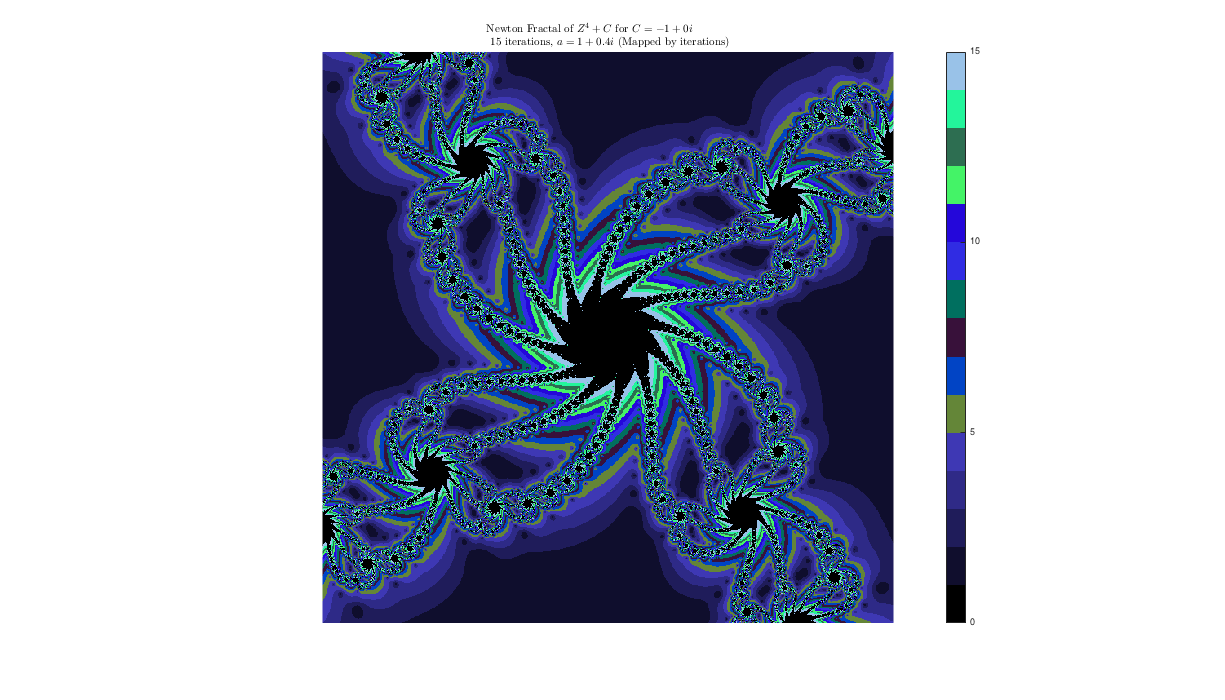
\includegraphics[width=0.7\linewidth]{images/goodImage3}
	\caption{}
	\label{fig:rootEx2}
\end{figure}
To map by iteration, we proceed with Newton’s method.  After each iteration, we check if the distance moved by each point is less than a given tolerance, implying that it has converged.  If so, that point is labeled with the current iteration count, and removed from the set for all following iterations. This method does not show which root to which a point converges, but it does show how long it takes for each point to converge.  This is useful for analyzing factors that may affect the rate of convergence for Newton’s method, namely roots with multiplicity greater than one. (a bit more detail to come)

%%%%%%%%%%%%%%%%%%%%%%%%%%%%%%%%%%%%%%%%%%%%%%%
\end{onehalfspace}
\pagebreak
\normalsize
\begin{center}
	\section*{Appendix}
\end{center}
\section*{References}
\begin{itemize}
	\item\url{https://www.mcgoodwin.net/julia/juliajewels.html}
	\item\url{http://math.bu.edu/DYSYS/FRACGEOM/node4.html}
	\item\url{http://lodev.org/cgtutor/juliamandelbrot.html}
	\item\url{http://www.relativitybook.com/CoolStuff/julia_set.html}
	\item\url{http://mrob.com/pub/muency/escaperadius.html}
	\item\url{http://www.dartmouth.edu/~michaeldowns/writeup.pdf}
	\item\url{https://www.whitman.edu/Documents/Academics/Mathematics/burton.pdf}
	\item\url{https://www.mitchr.me/SS/newton/#firstprogram}
	\item\url{http://www.chiark.greenend.org.uk/~sgtatham/newton}
	\item\url{http://atmos.eas.cornell.edu/~mek236/fractal}
	\item\url{http://young.physics.ucsc.edu/242/newton.pdf}
\end{itemize}
\subsection*{Proof 1: Powers of Complex Numbers}
\begin{center}
	Let $z= a + bi\hspace{10mm}|z|=r$\linebreak
	Since $z$ is complex, it can be written as $z=r(\cos\theta+i\sin\theta)$ for some $\theta$
	$$e^{ix} = \cos x+i\sin x$$
	$$(e^{ix})^n = (\cos x+i\sin x)^n = e^{nix} = \cos nx+i\sin nx$$
	$$z^n=r^n(\cos\theta+i\sin\theta)^n$$
	$$z^n=r^n(\cos n\theta+i\sin n\theta)$$
	$$|z^n|=|r^n(\cos n\theta+i\sin n\theta)|$$
	$$ = r^n|\cos n\theta+i\sin n\theta|$$
	$$ = r^n\hspace{10mm}\text{via Pythagorean Theorem}$$
	$$\huge\therefore\normalsize\hspace{5mm}|z^n|=|z|^n$$
\end{center}
\end{document}
